\chapter{Umsetzung des Projektes}
\section{Komponenten und Aufbau}
\label{sec:Peri}
Das Projekt wird auf einem Arduino Micro umgesetzt. Dieser ist ein Entwicklerboard, basierend auf dem Mikrocontroller ATmega32U4. Er wird mit 16MHz getaktet und 5V betrieben. Der Programmspeicher umfasst 32KB. Weiterhin besitzt der Controller 2.5KB SRAM als Arbeitsspeicher sowie 1KB EEPROM für dauerhaftes Speichern von Werten.
Die Steuerung des Spiels erfolgt über Joysticks, dessen Position über Potentiometer in eine Spannung abgebildet wird. 
Die Anzeige erfolgt über ein 4-Zeilen Display (Modell 2004) mit parallelem Interface. Ein FC-113 I2C-Brückenchip wandelt die seriell über I2C gesendeten Displaykommandos in das parallel Interface um. Das Programm wird mittels Programmer EvUSBasp auf den Controller geladen. Im Folgenden sind die verwendeten Komponenten aufgezählt:
\begin{enumerate}
\item Arduino Micro
\item I2C Displayinterface FC-113 
\item 4-Zeilen LC-Display Modell 2004
\item 2 $\times$ Potentiometer-Joystick
\item EvUSBasp USB-Programmer
\end{enumerate}

Abbildung \ref{fig:Aufbau} zeigt den Aufbau des Projektes.
\begin{figure}[H]
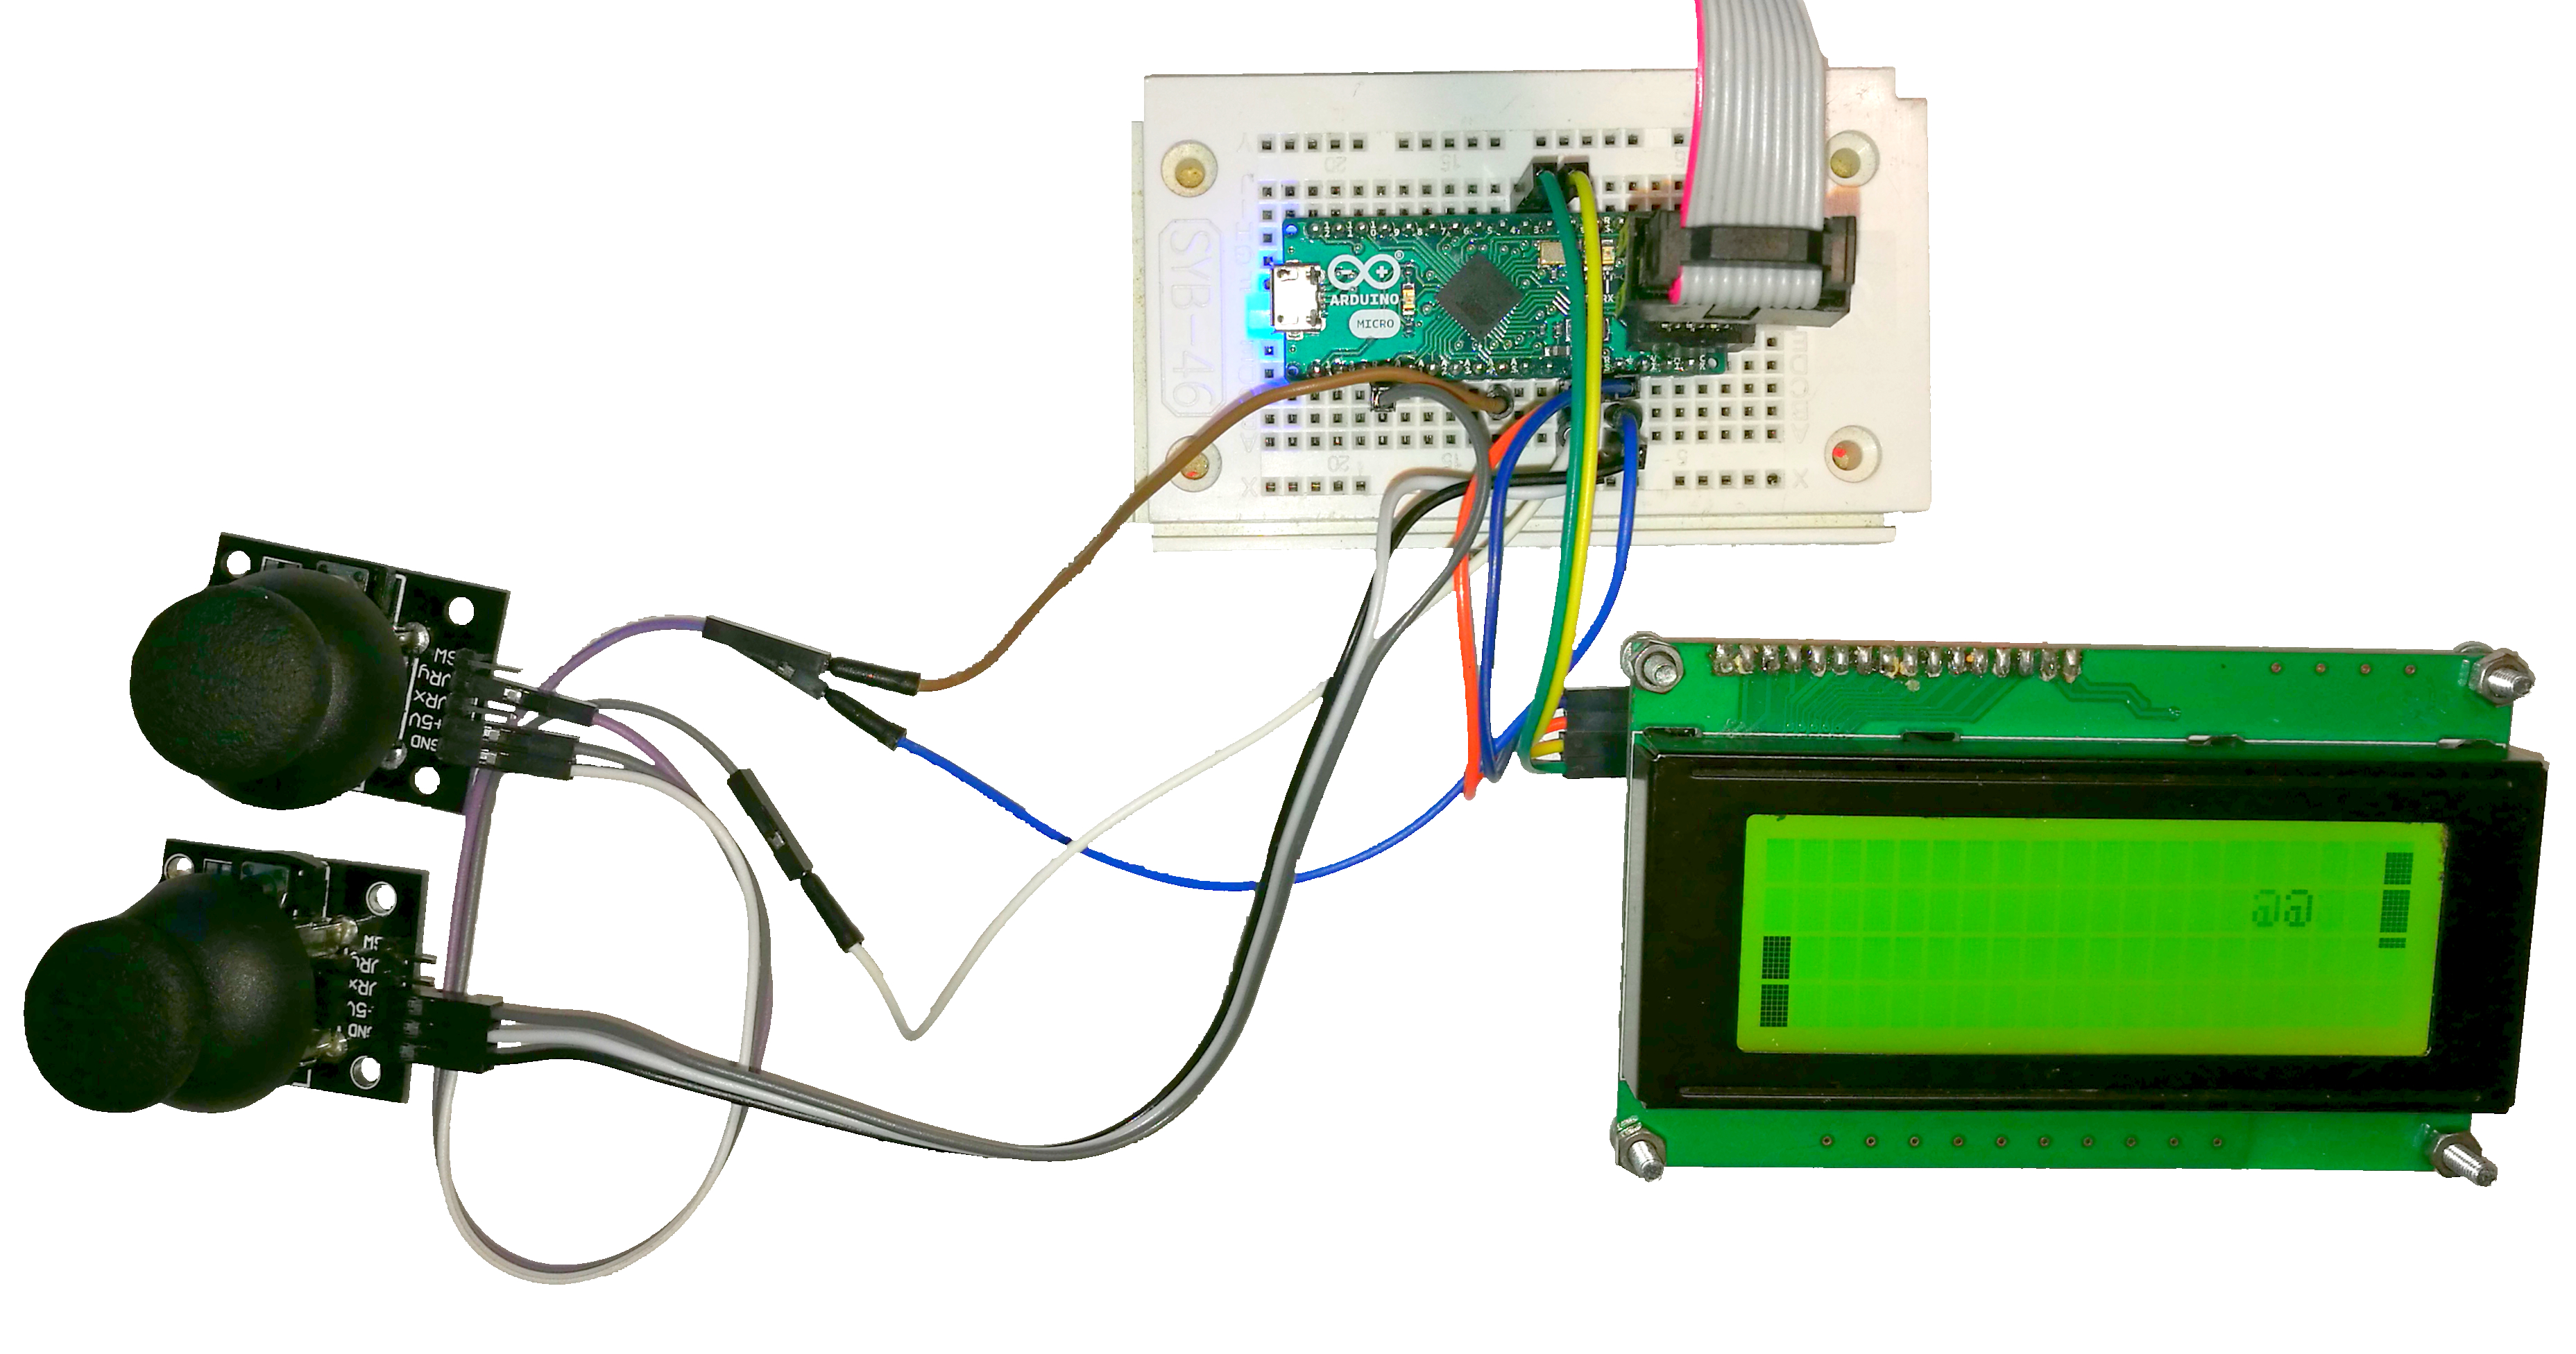
\includegraphics[width=\textwidth]{./Bilder/Aufbau.jpg}
\caption{Aufbau des Projektes}
\label{fig:Aufbau}
\end{figure}

Die nachfolgende Abbildung zeigt den zugehörigen Schaltplan. Er ist konsistent mit den im Programm deklarierten Pins.
\begin{figure}[H]
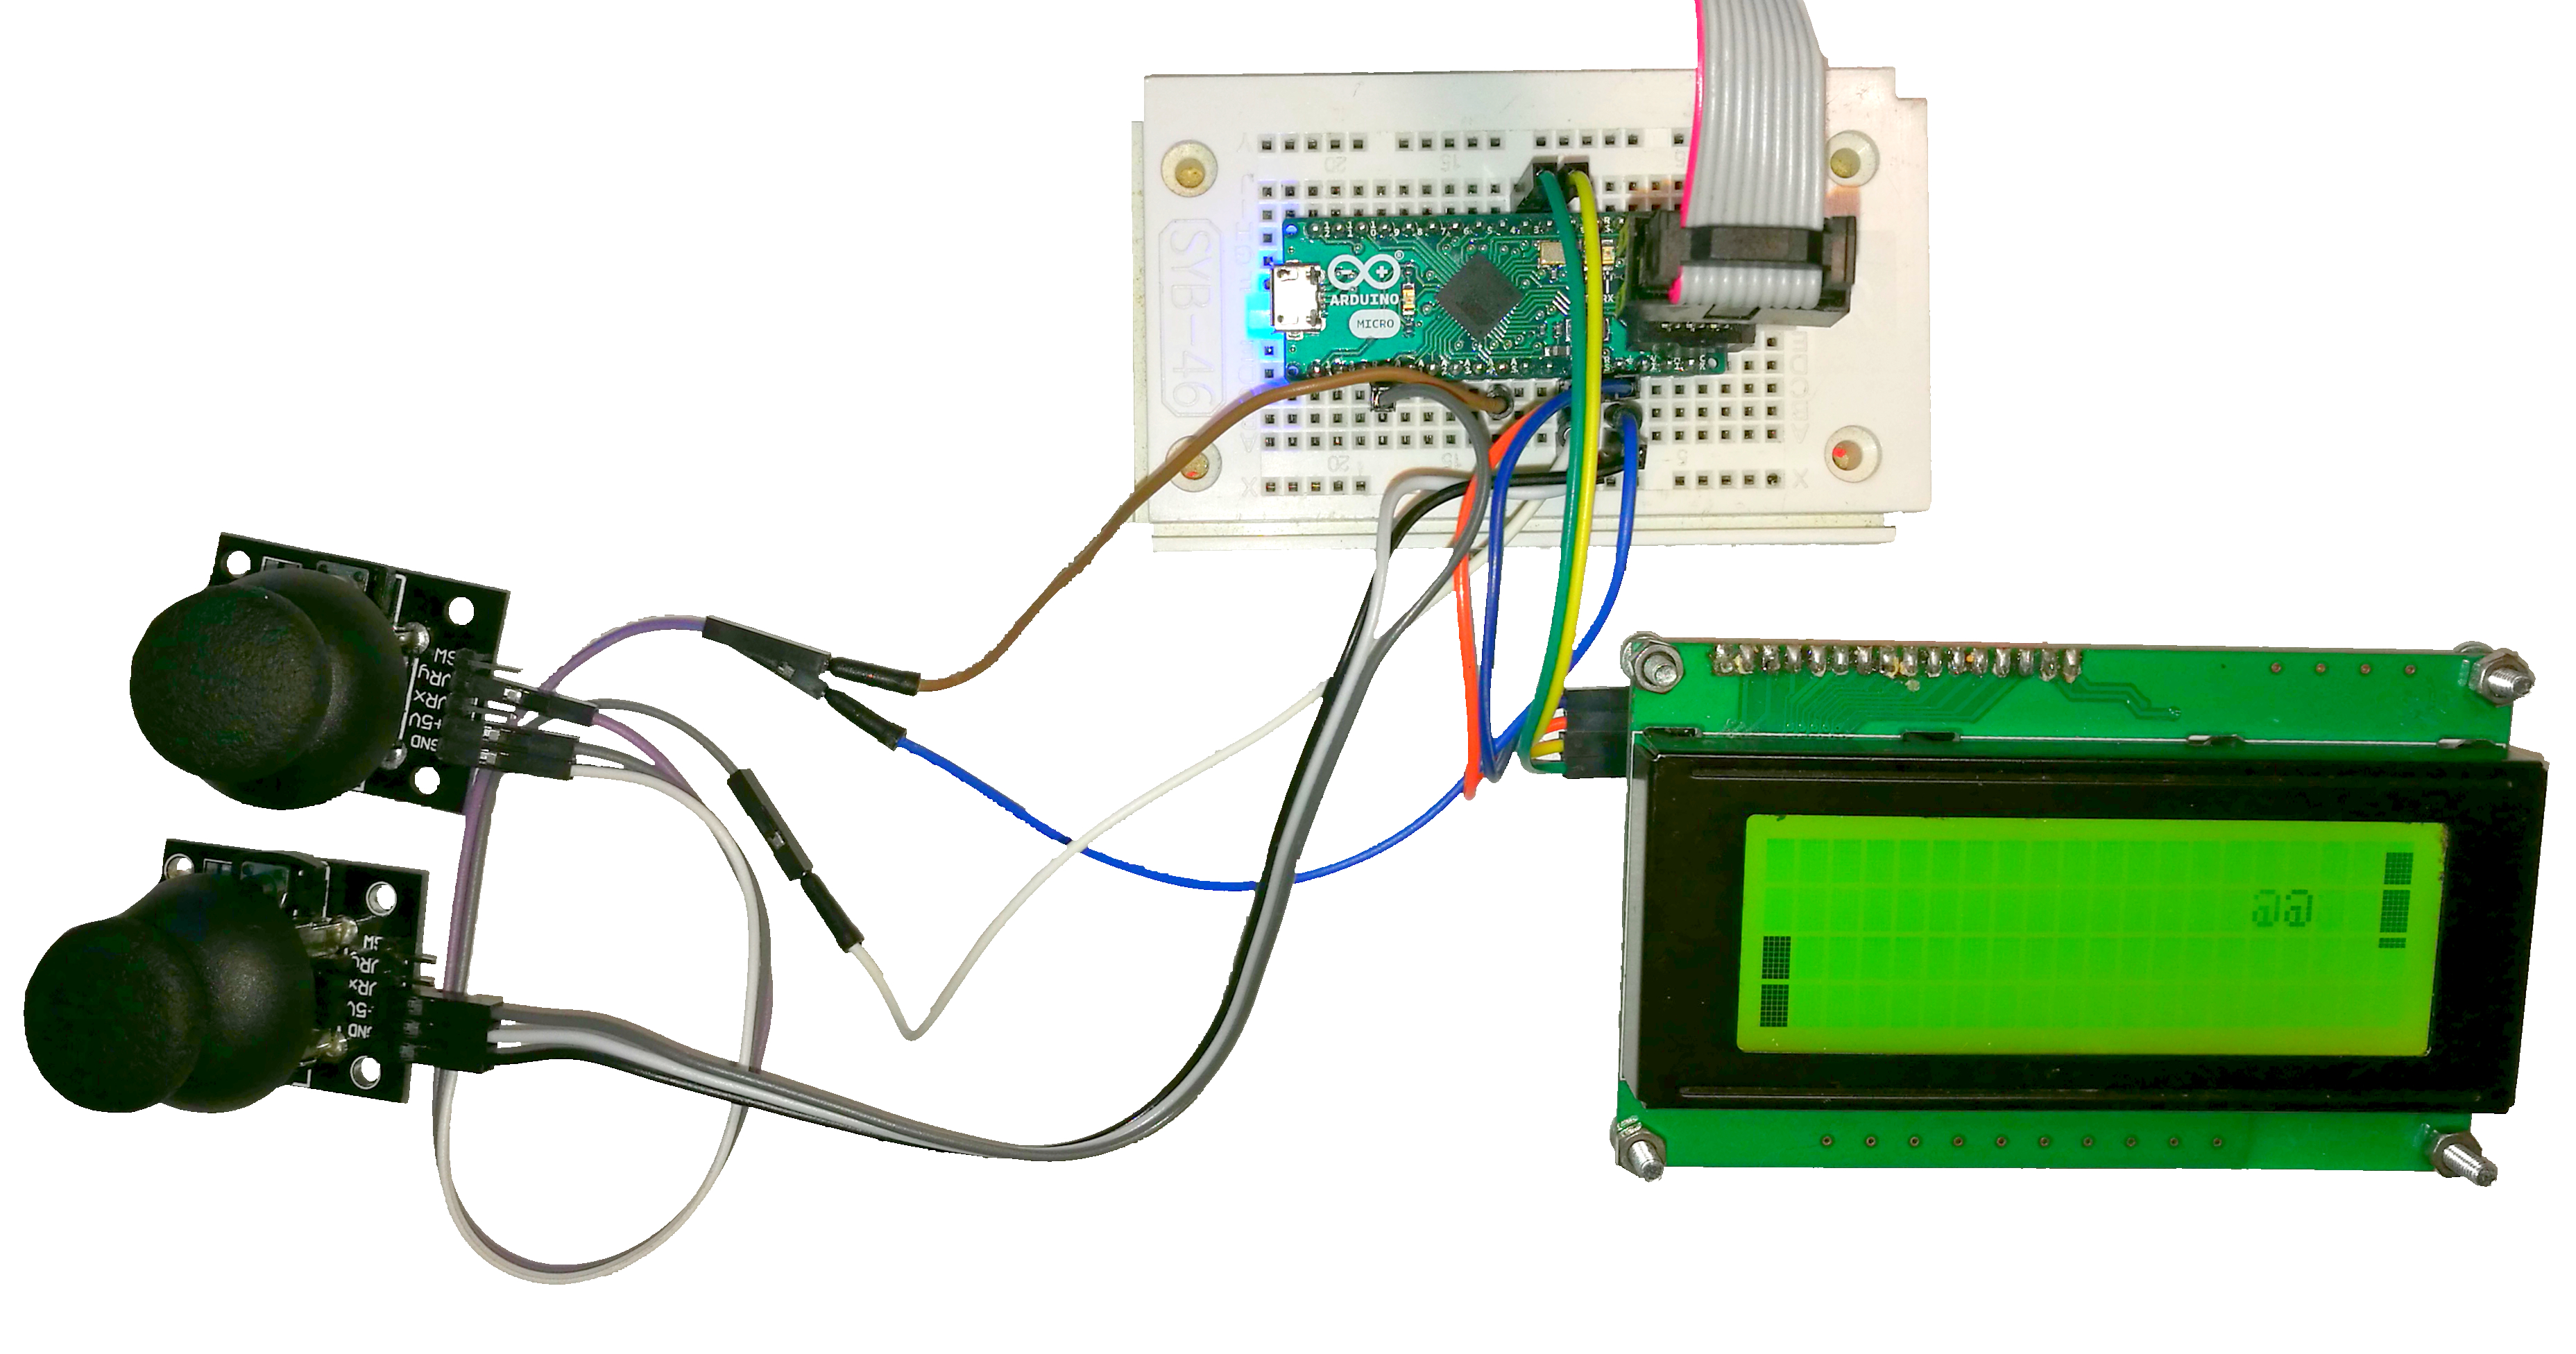
\includegraphics[width=\textwidth]{./Bilder/Aufbau.jpg}
\caption{Schaltplan des Projektes}
\label{fig:Schaltplan}
\end{figure}

\section{Einrichtung der Programmierumgebung}
\label{sec:IDE}
%oberfläche VS Code

\section{Programmstruktur}
\label{sec:Prog}
%was wird gemacht
%welche programmbestandteile
%verweis auf doxy doku im anhang

\section{Automatische Maschinencodeerstellung mittels Makefile}
\label{sec:Make}


 

